\section{Backtracking (Podas)}

	La descripción del problema como la forma de pensarlo son las mismas que el ejercicio anterior.

\subsection{Resolución}
	
	Además de lo dicho en el ejercicio anterior, la idea es podar más el árbol para no recorrer ramas donde no nos interese su solución o sea un caso inválido. Para esto tenemos 2 podas, la primera consiste en no ramas que no mejoren mi mejor solución hasta el momento y la segunda consiste en hacer un análisis a futuro de la confiabilidad de los agentes. Para la primera consideremos un conjunto con "k" elementos en el, "a" representa la cantidad total de agentes e "i" representa los agentes que ya fueron evaluados, la poda consiste en que si $k+(a-i)$ <= s (notar que "a-i" representa los agentes que faltan por evaluar), donde s es la mejor solución hasta el momento, si esto pasa no seguimos recorriendo esa rama ya que no aporta nada mejor a lo que tenemos. La otra consiste en hacer un mejor chequeo de la confiabilidad. Además de lo descripto en el ejercicio anterior, vemos que si el agente a ser agregado, llamemoslo "x", confia en otro agente "y", "y" pueda formar parte del conjunto.  Para esto vereficamos la confiabilidad de "y" si resulta que no podemos agregarlo al conjunto tampoco agregamos a "x" por lo que no recorremos esa posibilidad. 
	
\subsection{Pseudocódigo}  
	
\begin{algorithm}[H]
\caption{BacktrackingPodas}\label{Ej1.1}

\begin{algorithmic}[H]
\Procedure{BacktrackingPodas}{vector(pair(agente, agente)) encuestas, agentes, ConjAgentes}
\If{Si no me quedan agentes para evaluar}
\If{longitud(ConjAgentes) > solucion}
\State solucion $=$ longitud(ConjAgentes)
\EndIf
\State\Return solucion
\EndIf
\If{PuedoAgregarAgente $\wedge$ PuedeSerMejorSolución}
\State Paso Recursivo rama agregueAlAgente
\EndIf
\If{PuedeSerMejorSolución}
\State Paso Recursivo rama NoAgregoAlAgente
\EndIf
\EndProcedure
\end{algorithmic}

\end{algorithm}

\subsection{Complejidad}

	Dado que las podas no agregan complejidad al algoritmo ya que se aprovechan de lo que se hacía antes y en peor caso tengo que recorrer todo el árbol, la complejidad en peor caso sigue siendo lo misma que el ejercicio anterior. O($2^{i}*i^{3}*a^{3}$). 
	
\subsection{Experimentación}

\begin{figure}[h]

\begin{subfigure}{0.5\textwidth}
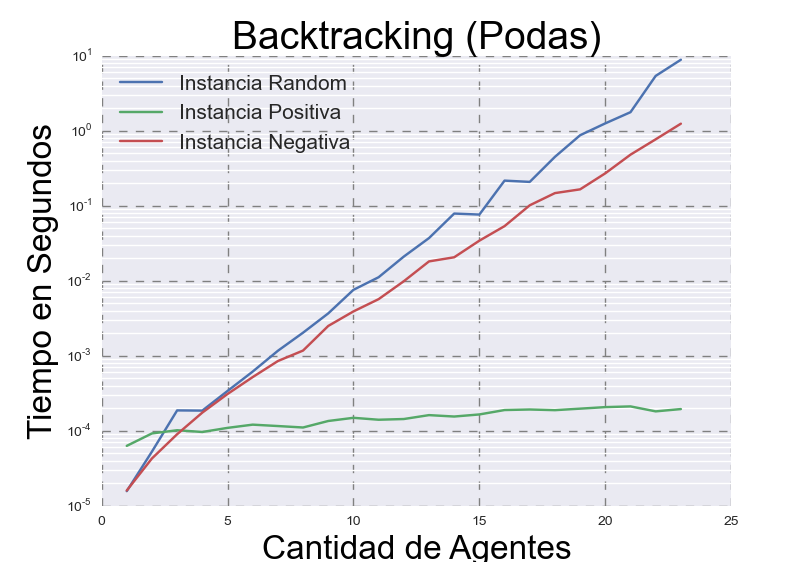
\includegraphics[scale=0.45]{PodasLog.png}
\end{subfigure}
\begin{subfigure}{0.5\textwidth}
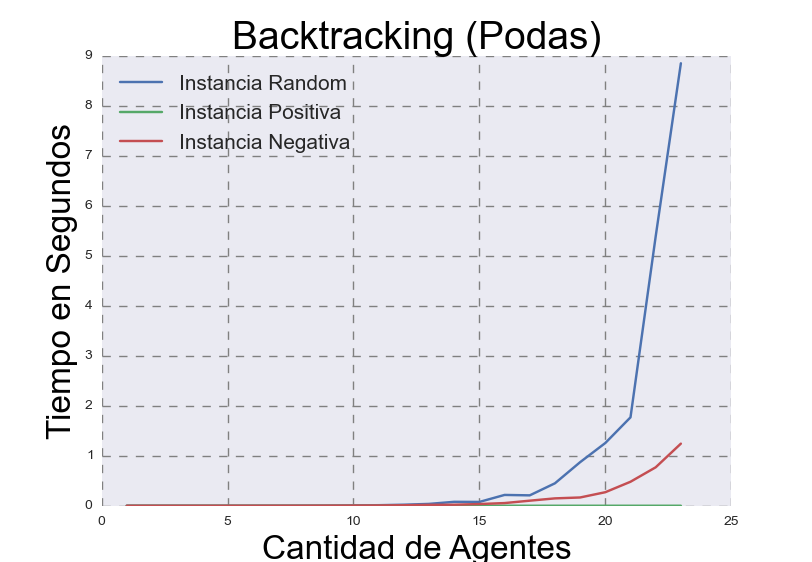
\includegraphics[scale=0.45]{Podas.png}
\end{subfigure}

\end{figure}

	Al igual que en el ejercicio anterior vemos los resultados del algoritmo para diferentes entradas. La muestras fueron calculadas de la misma manera que en el ejercicio anterior.